\documentclass{article}
\usepackage{amsmath}
\usepackage{amssymb}
\usepackage{graphicx}
\usepackage{hyperref}
\usepackage[version=4]{mhchem}

\title{Problem 3}
\date{}

\begin{document}
\maketitle

\section*{Problem}
As shown in the figure, \(A B\) is the diameter of a semicircle and \(C D\) is a chord parallel to \(A B\). Connect \(A D\) and extend it to meet \(B E\) of the perpendicular of \(A B\) at \(E\). Draw \(E F \perp A C\) and meets the extension of \(A C\) at \(F, F\) is the foot of perpendicular. Show that \(A C=C F\).\\
\centering
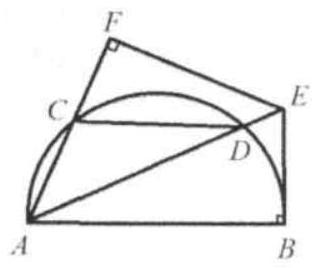
\includegraphics[width=\textwidth]{images/problem_image_1.jpg}

\section*{Solution}
Since \(\angle F=\angle B=90^{\circ}\), points \(A, B, E\), and \(F\) are concyclic.\\
\(\angle A F B=\angle A E B=\gamma\).\\
Since \(C D / / A B\), arcs \(A C=B D, \angle D A B=\angle C B A=\alpha\).\\
In Rt \(\triangle A B E, \alpha+\gamma=90^{\circ}\).\\
\centering
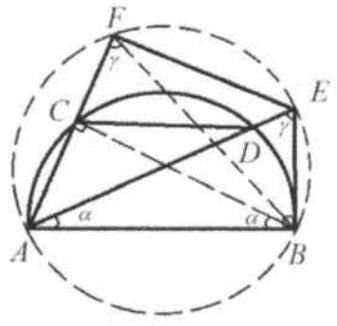
\includegraphics[width=\textwidth]{images/reasoning_image_1.jpg}

In Rt \(\triangle B C F, \angle F B C+\gamma=90^{\circ}\). So \(\angle F B C=\alpha\). \(B C\) is the perpendicular bisector of \(A F\) in \(\triangle B A F\). So \(A C=C F\).

\end{document}
